\newcommand{\gridsansowners}{
  % grid
  \draw[line width=1.0pt] (0.0,0.0) -- (0.0,1.0) -- (1.0,1.0) -- (1.0,0.0) -- cycle;
  \pgfmathsetmacro\fifth{1.0/5.0}
  \draw[xstep=\fifth,ystep=\fifth,black,thin] (0.0,0.0) grid (1.0,1.0);
  % prominent nodes
  \foreach \x in {1,...,4} {
    \foreach \y in {1,...,4} {
        \filldraw (\x * \fifth,\y * \fifth) circle (0.4pt);
    }
  }
  % tick marks for i
  \draw[line width=1.0pt] (0.2,-0.04) -- (0.2,0.02);
  \draw[line width=1.0pt] (0.8,-0.04) -- (0.8,0.02);
  \node[yshift=-4mm] at (0.2,0.0) {\small $i=0$};
  \node[yshift=-4mm] at (0.8,0.0) {\small $m_x\!-\!1$};
  % tick marks for j
  \draw[line width=1.0pt] (-0.04,0.2) -- (0.02,0.2);
  \draw[line width=1.0pt] (-0.04,0.8) -- (0.02,0.8);
  \node[xshift=-6mm] at (0.0,0.2) {\small $j=0$};
  \node[xshift=-6.5mm] at (0.0,0.8) {\small $m_y\!-\!1$};
}

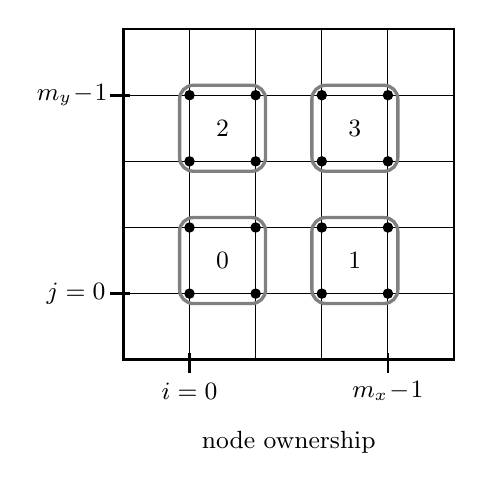
\begin{tikzpicture}[scale=4.2]
\gridsansowners
\pgfmathsetmacro\half{0.5*\fifth}
\pgfmathsetmacro\AA{0.15*\fifth}
\foreach \x in {1,3} {
    \foreach \y in {1,3} {
        \draw[very thick,rounded corners=5pt,gray] (\x*\fifth-\AA,\y*\fifth-\AA) -- (\x*\fifth+\fifth+\AA,\y*\fifth-\AA) -- (\x*\fifth+\fifth+\AA,\y*\fifth+\fifth+\AA) -- (\x*\fifth-\AA,\y*\fifth+\fifth+\AA) -- cycle;
    }
}
\node at (\fifth+\half,\fifth+\half) {\small $0$};
\node at (3*\fifth+\half,\fifth+\half) {\small $1$};
\node at (\fifth+\half,3*\fifth+\half) {\small $2$};
\node at (3*\fifth+\half,3*\fifth+\half) {\small $3$};
\node at (0.5,-0.25) {\small node ownership};
\end{tikzpicture}
\quad
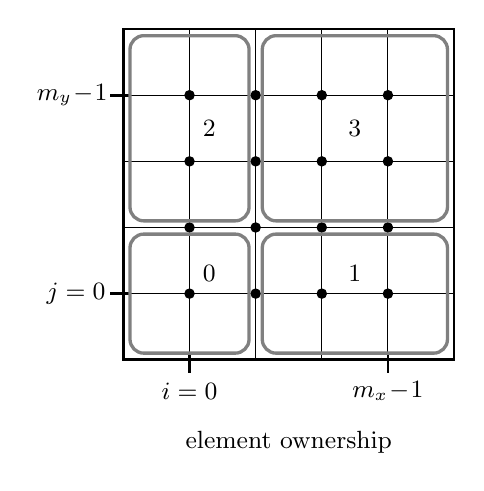
\begin{tikzpicture}[scale=4.2]
\gridsansowners
\pgfmathsetmacro\half{0.5*\fifth}
\pgfmathsetmacro\bit{0.3*\fifth}
\pgfmathsetmacro\BB{0.1*\fifth}
\draw[very thick,rounded corners=5pt,gray] (\BB,\BB) -- (2*\fifth-\BB,\BB) -- (2*\fifth-\BB,2*\fifth-\BB) -- (\BB,2*\fifth-\BB) -- cycle;
\draw[very thick,rounded corners=5pt,gray] (2*\fifth+\BB,\BB) -- (5*\fifth-\BB,\BB) -- (5*\fifth-\BB,2*\fifth-\BB) -- (2*\fifth+\BB,2*\fifth-\BB) -- cycle;
\draw[very thick,rounded corners=5pt,gray] (\BB,2*\fifth+\BB) -- (2*\fifth-\BB,2*\fifth+\BB) -- (2*\fifth-\BB,5*\fifth-\BB) -- (\BB,5*\fifth-\BB) -- cycle;
\draw[very thick,rounded corners=5pt,gray] (2*\fifth+\BB,2*\fifth+\BB) -- (5*\fifth-\BB,2*\fifth+\BB) -- (5*\fifth-\BB,5*\fifth-\BB) -- (2*\fifth+\BB,5*\fifth-\BB) -- cycle;
\node at (\fifth+\bit,\fifth+\bit) {\small $0$};
\node at (3*\fifth+\half,\fifth+\bit) {\small $1$};
\node at (\fifth+\bit,3*\fifth+\half) {\small $2$};
\node at (3*\fifth+\half,3*\fifth+\half) {\small $3$};
\node at (0.5,-0.25) {\small element ownership};
\end{tikzpicture}

